\documentclass{article}
% Language setting
% Replace `english' with e.g. `spanish' to change the document language
\usepackage{biblatex} %Imports biblatex package
\addbibresource{sample.bib}
\usepackage{changepage}
\usepackage[english]{babel}
\usepackage{tikz}
\usepackage{array}
\usepackage{amsmath}
\usepackage{accents}
\usepackage{empheq}
\usepackage{pythonhighlight}
\newcolumntype{P}[1]{>{\centering\arraybackslash}p{#1}}
\newcolumntype{M}[1]{>{\centering\arraybackslash}m{#1}}

% Set page size and margins
% Replace `letterpaper' with `a4paper' for UK/EU standard size
\usepackage[letterpaper,top=2cm,bottom=2cm,left=3cm,right=3cm,marginparwidth=1.75cm]{geometry}

\usepackage{graphicx}
\usepackage[colorlinks=true, allcolors=blue]{hyperref}
\usepackage{setspace}
\usepackage{booktabs}
\usepackage[T1]{fontenc}
\usepackage{longtable}
\doublespacing

\begin{document}
\newcommand{\circled}[1]{\tikz[baseline=(char.base)]{
            \node[shape=circle,draw,inner sep=2pt] (char) {#1};}}

\newcommand{\pd}[3]{\frac{\partial^{#3}#1}{\partial {#2}^{#3}}}
\begin{titlepage}

\centering
\scshape
\vspace{\baselineskip}

%
\rule{\textwidth}{1.6pt}\vspace*{-\baselineskip}\vspace*{2pt}
\rule{\textwidth}{0.4pt}

{\Huge \textbf{\textsc{NPRE 449: Homework 10 \\
\vspace{15pt}}}}

\rule{\textwidth}{0.4pt}\vspace*{-\baselineskip}\vspace{3.2pt}
\rule{\textwidth}{1.6pt}\vspace{6pt}
%%\centerline{\textit{University of Illinois at Urbana-Champaign}} 
\vspace{1.5\baselineskip}


\large \centerline{\textbf{Author:} Nathan Glaser}
\large \centerline{\textbf{Net-ID:} nglaser3}
\quad

\vfill
\large \centerline{December 4, 2024}
%
\pagenumbering{gobble}
\end{titlepage}

\tableofcontents
\newpage
\pagenumbering{arabic}

\section{Question 1}
To begin, the area averaged equations are:
\begin{subequations}
    \begin{equation}
        \pd{\rho}{t}{} + \pd{\rho v}{z}{} = 0
        \label{mass}
    \end{equation}
    \begin{equation}
        \pd{\rho v}{t}{} + \pd{}{z}{}\rho v^2 = -\pd{P}{z}{}-\tau_F\frac{\xi_w}{A_f} - \rho g \sin(\theta)
        \label{momentum}
    \end{equation}
    \begin{equation}
        \pd{\rho h}{t}{} + \pd{}{z}{}\rho v h = \frac{q''\xi_h}{A}+\pd{P}{t}{} + q'''
        \label{energy}
    \end{equation}
\end{subequations}

Then, our problem is steady-state, and has constant material properties and no heat generation in the fluid. Further, substituting $\rho v$ as $G$, we obtain our base equations for this problem.

\begin{subequations}
    \begin{equation}
        \pd{G}{z}{} = 0
        \label{mass}
    \end{equation}
    \begin{equation}
         -\pd{P}{z}{} = G^2\pd{}{z}{}\frac{1}{\rho} + \tau_F\frac{\xi_w}{A_f} + \rho g 
        \label{momentum}
    \end{equation}
    \begin{equation}
        G\pd{}{z}{} h = \frac{q''\xi_h}{A}
        \label{energy}
    \end{equation}
\end{subequations}

Then, converting $h$ for the equilibrium steam quality, $\chi_e$, and substituting into the energy equation:

\begin{subequations}
    \begin{equation}
        h = h_f + h_{fg}\chi_e
    \end{equation}
    \begin{equation}
        \pd{}{z}{}h =  h_{fg}\pd{}{z}{} \chi_e
    \end{equation}
\end{subequations}

thus: 

\begin{equation}
    \pd{}{z}{}\chi_e = \frac{q''\xi_h}{Gh_{fg}A}
\end{equation}

Thus, because the heat flux is constant, we integrate both sides and solve:

\begin{equation}
    \chi_e = \chi_{e,0} + \frac{q''\xi_h}{Gh_{fg}A} z
\end{equation}

Then, investigating the momentum equation, recognizing $\chi = \chi_e$ for this problem and changing $\rho$ to $\rho_m$:
\begin{subequations}
    \begin{equation}
        \rho_m = \biggr( \frac{1}{\rho_f} + \frac{\chi}{\rho_{fg}} \biggr)^{-1}
    \end{equation}
    \begin{equation}
        \pd{}{z}{}\frac{1}{\rho_m} = \frac{1}{\rho_{fg}}\pd{}{z}{}\chi =  \frac{q''\xi_h}{\rho_{fg}Gh_{fg}A}
    \end{equation}
    \begin{equation}
        -\pd{P}{z}{} = \frac{Gq''\xi_h}{\rho_{fg}Gh_{fg}A} + \tau_F\frac{\xi_w}{A_f} +  \biggr( \frac{1}{\rho_f} + \frac{\chi}{\rho_{fg}} \biggr)^{-1} g
    \end{equation}
\end{subequations}

Finally, solving, for the pressure drop (substituting $\tau_F = \frac{fG^2}{2\rho_m}$):

\begin{subequations}
    \begin{equation}
        -\pd{P}{z}{} = \frac{Gq''\xi_h}{\rho_{fg}Gh_{fg}A} + \frac{fG^2\xi_w}{2A_f}\bigr(V_f+V_{fg}\chi_e\bigr) + \biggr( \frac{1}{\rho_f} + \frac{\chi}{\rho_{fg}} \biggr)^{-1} g 
    \end{equation}
    \begin{equation}
        -\int_0^z\partial P = \int_0^z\biggr(\frac{Gq''\xi_h}{\rho_{fg}Gh_{fg}A} + \frac{fG^2\xi_w}{2A_f}\bigr(V_f+V_{fg}\chi_e\bigr) + \biggr( \frac{1}{\rho_f} + \frac{\chi}{\rho_{fg}} \biggr)^{-1} g\biggr)\partial z
    \end{equation}
    \begin{equation}
        \Delta P = \biggr(\frac{Gq''\xi_h}{\rho_{fg}Gh_{fg}A}\biggr)\cdot L + 
        \frac{fG^2\xi_w}{2A_f}\int_0^L\bigr(V_f+V_{fg}\chi_e\bigr)\partial z
        +g\int_0^L \biggr( \frac{1}{\rho_f} + \frac{\chi}{\rho_{fg}} \biggr)^{-1} \partial z
    \end{equation}
    \begin{equation}
        \int_0^Lh_{fg}\chi_e = V_{fg}\chi_{e,0}L + \frac{V_{fg}q''\xi_h}{Gh_{fg}A} L^2
    \end{equation}
    Setting $u = \frac{1}{\rho_f} + \frac{\chi}{\rho_{fg}}$, and $du = \frac{\rho_{fg}Gh_{fg}A}  {q''\xi_h}\partial z$
    \begin{equation}
        \frac{\rho_{fg}Gh_{fg}A}{q''\xi_h}\int_0^L  u ^{-1} \partial u = \frac{\rho_{fg}Gh_{fg}A}{q''\xi_h}\ln{u} = \frac{\rho_{fg}Gh_{fg}A}{q''\xi_h}\ln\bigr( V_f + V_{fg}\frac{q''\xi_h}{Gh_{fg}A}L + \chi_{e,0}L\bigr)
    \end{equation}
    \begin{equation}
        \Delta P = \biggr(\frac{Gq''\xi_h}{\rho_{fg}Gh_{fg}A}\biggr)\cdot L + \frac{fG^2\xi_w}{2A_f}\biggr(V_fL+V_{fg}\chi_{e,0}L + \frac{V_{fg}q''\xi_h}{Gh_{fg}A} L^2\biggr) + \frac{\rho_{fg}Gh_{fg}A}{q''\xi_h}\ln\bigr( V_f + V_{fg}\frac{q''\xi_h}{Gh_{fg}A}L + \chi_{e,0}L\bigr)
    \end{equation}
\end{subequations}
And because $\chi_e$ at 0 is 0:

\begin{equation}
    \Delta P = \biggr(\frac{Gq''\xi_h}{\rho_{fg}Gh_{fg}A}\biggr)\cdot L + \frac{fG^2\xi_w}{2A_f}\biggr(V_fL + \frac{V_{fg}q''\xi_h}{Gh_{fg}A} L^2\biggr)+ \frac{\rho_{fg}Gh_{fg}A}{q''\xi_h}\ln\bigr( V_f + V_{fg}\frac{q''\xi_h}{Gh_{fg}A}L\bigr)
\end{equation}

This would change simply by flipping the sign of the $\rho g$:
\begin{equation}
    \Delta P = \biggr(\frac{Gq''\xi_h}{\rho_{fg}Gh_{fg}A}\biggr)\cdot L + \frac{fG^2\xi_w}{2A_f}\biggr(V_fL + \frac{V_{fg}q''\xi_h}{Gh_{fg}A} L^2\biggr)
\end{equation}

\newpage
\section{Question 2}
The problem statement is essentially identical to the previous, atleast similair enough where our base equations are the same:
\begin{subequations}
    \begin{equation}
        \pd{G}{z}{} = 0
    \end{equation}
    \begin{equation}
        -\pd{P}{z}{} = G^2\pd{}{z}{}\frac{1}{\rho_m} + \frac{fG^2\xi_w}{2A_f}\rho_m
    \end{equation}
    \begin{equation}
    \pd{}{z}{}\chi_e = \frac{q''\xi_h}{Gh_{fg}A}
    \end{equation}
\end{subequations}

First, solving for the steam quality. For all three cases, the heat flux takes the form of $q_m''z + q_0''$, where $q_m''$ is the slope of the heat flux line in z, and $q_0''$ is the initial heat flux at the inlet. Thus solving:

\begin{subequations}
    \begin{equation}
        \int_0^z\partial\chi = \int_0^z\frac{q''\xi_h}{Gh_{fg}A}\partial z
    \end{equation}
    \begin{equation}
        \int_0^z\partial\chi = \frac{\xi_h}{Gh_{fg}A}\int_0^z\bigr(q_m''z + q_0''\bigr)\partial z
    \end{equation}
    \begin{equation}
        \chi = \frac{\xi_h}{Gh_{fg}A}\bigr(\frac{q_m''}{2}z^2 + q_0''z\bigr)
    \end{equation}
\end{subequations}

Proximally, substituting $\chi$ into $\rho_m$, and solving for the pressure drop for the flat case:

\begin{subequations}
    \begin{equation}
        -\pd{P}{z}{} = G^2\pd{}{z}{}\bigr(V_f+V_{fg}\chi_e\bigr) + \frac{fG^2\xi_w}{2A_f}\bigr(V_f+V_{fg}\chi_e\bigr)
    \end{equation}
    \begin{equation}
        -\pd{P}{z}{} = G^2V_{fg}\frac{\xi_h}{Gh_{fg}A}\bigr(q_m''z + q_0''\bigr) + \frac{fG^2\xi_w}{2A_f}\bigr(V_f+V_{fg}\chi_e\bigr)
    \end{equation}
    \begin{equation}
        -\int_0^L\partial P = \int_0^L\biggr( G^2V_{fg}\frac{\xi_h}{Gh_{fg}A}\bigr(q_m''z + q_0''\bigr) + \frac{fG^2\xi_w}{2A_f}\bigr(V_f+V_{fg}\frac{\xi_h}{Gh_{fg}A}\bigr(\frac{q_m''}{2}z^2 + q_0''z\bigr)\bigr) \biggr)\partial z
    \end{equation}
    \begin{equation}
        \Delta P = G^2V_{fg}\frac{\xi_h}{Gh_{fg}A}\bigr(\frac{q_m''}{2}L^2 + q_0''L\bigr) + \frac{fG^2\xi_w}{2A_f}\bigr(V_fL+V_{fg}\frac{\xi_h}{Gh_{fg}A}\bigr(\frac{q_m''}{6}L^3 + \frac{q_0''}{2}L^2\bigr)\bigr)
    \end{equation}
    \begin{equation}
    \boxed{
        \Delta P = \frac{fG\xi^2V_{fg}}{12A_fh_{fg}A}q_m''L^3 + \biggr(\frac{GV_{fg}\xi_hq_m''}{2h_{fg}A} + \frac{fG\xi^2V_{fg}}{4A_fh_{fg}A}q_0''\biggr)L^2 + 
        \biggr( \frac{GV_{fg}\xi_h}{h_{fg}A}q_0'' + \frac{fV_fG^2\xi_w}{2A_f}\biggr)L
        }
    \end{equation}
\end{subequations}
\subsection{Part A}
substituting $q_m''$ as 0:
\begin{equation}
    \boxed{
        \Delta P = \frac{fG\xi^2V_{fg}}{4A_fh_{fg}A}q_0''L^2 + 
        \biggr( \frac{GV_{fg}\xi_h}{h_{fg}A}q_0'' + \frac{fV_fG^2\xi_w}{2A_f}\biggr)L
        }
\end{equation}

\subsection{Part B}

substituting in $q_0''$ as 0:
\begin{equation}
    \boxed{
        \Delta P = \frac{fG\xi^2V_{fg}}{12A_fh_{fg}A}q_m''L^3 + \frac{GV_{fg}\xi_hq_m''}{2h_{fg}A}L^2 + 
        \frac{fV_fG^2\xi_w}{2A_f}L
    }
\end{equation}

\subsection{Part C}

For this case, neither components drop to 0, thus:

\begin{equation}
    \boxed{
        \Delta P = \frac{fG\xi^2V_{fg}}{12A_fh_{fg}A}q_m''L^3 + \biggr(\frac{GV_{fg}\xi_hq_m''}{2h_{fg}A} + \frac{fG\xi^2V_{fg}}{4A_fh_{fg}A}q_0''\biggr)L^2 + 
        \biggr( \frac{GV_{fg}\xi_h}{h_{fg}A}q_0'' + \frac{fV_fG^2\xi_w}{2A_f}\biggr)L
        }
\end{equation}

\section{Question 3}

To begin, our mass and energy equations are (applying steady state, no heat gen in water):

\begin{subequations}
    \begin{equation}
        \pd{G}{z}{} = 0
    \end{equation}
    \begin{equation}
        G \pd{h}{z}{} = \frac{q''\xi_h}{A}
    \end{equation}
\end{subequations}

where:
\begin{subequations}
    \begin{equation}
        h = h_f + h_{fg}\chi_e
    \end{equation}
    \begin{equation}
        \pd{h}{z}{} = h_{fg}\pd{\chi_e}{z}{}
    \end{equation}
\end{subequations}

Thus our energy equation is simply, and solved:

\begin{subequations}
    \begin{equation}
        \pd{\chi_e}{z}{} = \frac{q''\xi_h}{AGh_{fg}}
    \end{equation}
    \begin{equation}
        \chi_e = \frac{q''\xi_h}{AGh_{fg}} z + \chi_{e,0}
    \end{equation}
\end{subequations}

Then, the fluid temperature while sub cooled is:

\begin{equation}
    T_f = \frac{h_{fg}}{c_p}\chi_e + T_{sat}
\end{equation}

The heat transfer scheme for the code is:
\begin{subequations}
    \begin{equation}
        if\ Tw\ \leq\ T_sat:\: q'' = h(T_w - T_f),\: Dittus-Boelter
    \end{equation}
    \begin{equation}
        else:\: q'' =\left[ \{Fh_{fc}(T_w - T_f)v^2\} + \{ Sh_{nb}(T_w-T_{sat})\}^2\right]^{\frac{1}{2}}
    \end{equation}
\end{subequations}

where:
\begin{subequations}
    \begin{equation}
        F = \left[ 1+ \chi Pr_f (\frac{\rho_f}{\rho_g}- 1)\right]^{0.35}
    \end{equation}
    \begin{equation}
        S = (1 + 0.055F^{0.1}Re_f^{0.16})^{-1}
    \end{equation}
    \begin{equation}
        h_{fc} = 0.023\frac{k_f}{D_h}Re_f^{0.8}Pr_f^{0.4}
    \end{equation}
    \begin{equation}
        h_{nb} = 55 (\frac{P}{P_c})^{0.12}q''^{2/3}\left(-\log{\frac{P}{P_c}}\right)^{-.55} M_w^{-0.5}
    \end{equation}
    \begin{equation}
        Re_f = \frac{GD_h}{\mu_f}
    \end{equation}
\end{subequations}

To begin, utilizing \texttt{scipy.optimize.root} to determine the locations in which the steam quality is 0 and 1 yields:
\begin{table}[!hp!]
    \centering
    \begin{tabular}{c|c}
         $\chi_e$ & Axial Position [m] \\
         0.0 & 0.31505 \\
         1.0 & 11.59775
    \end{tabular}
\end{table}

And then, determining the wall temperature:

\begin{figure}[!hp!]
    \centering
    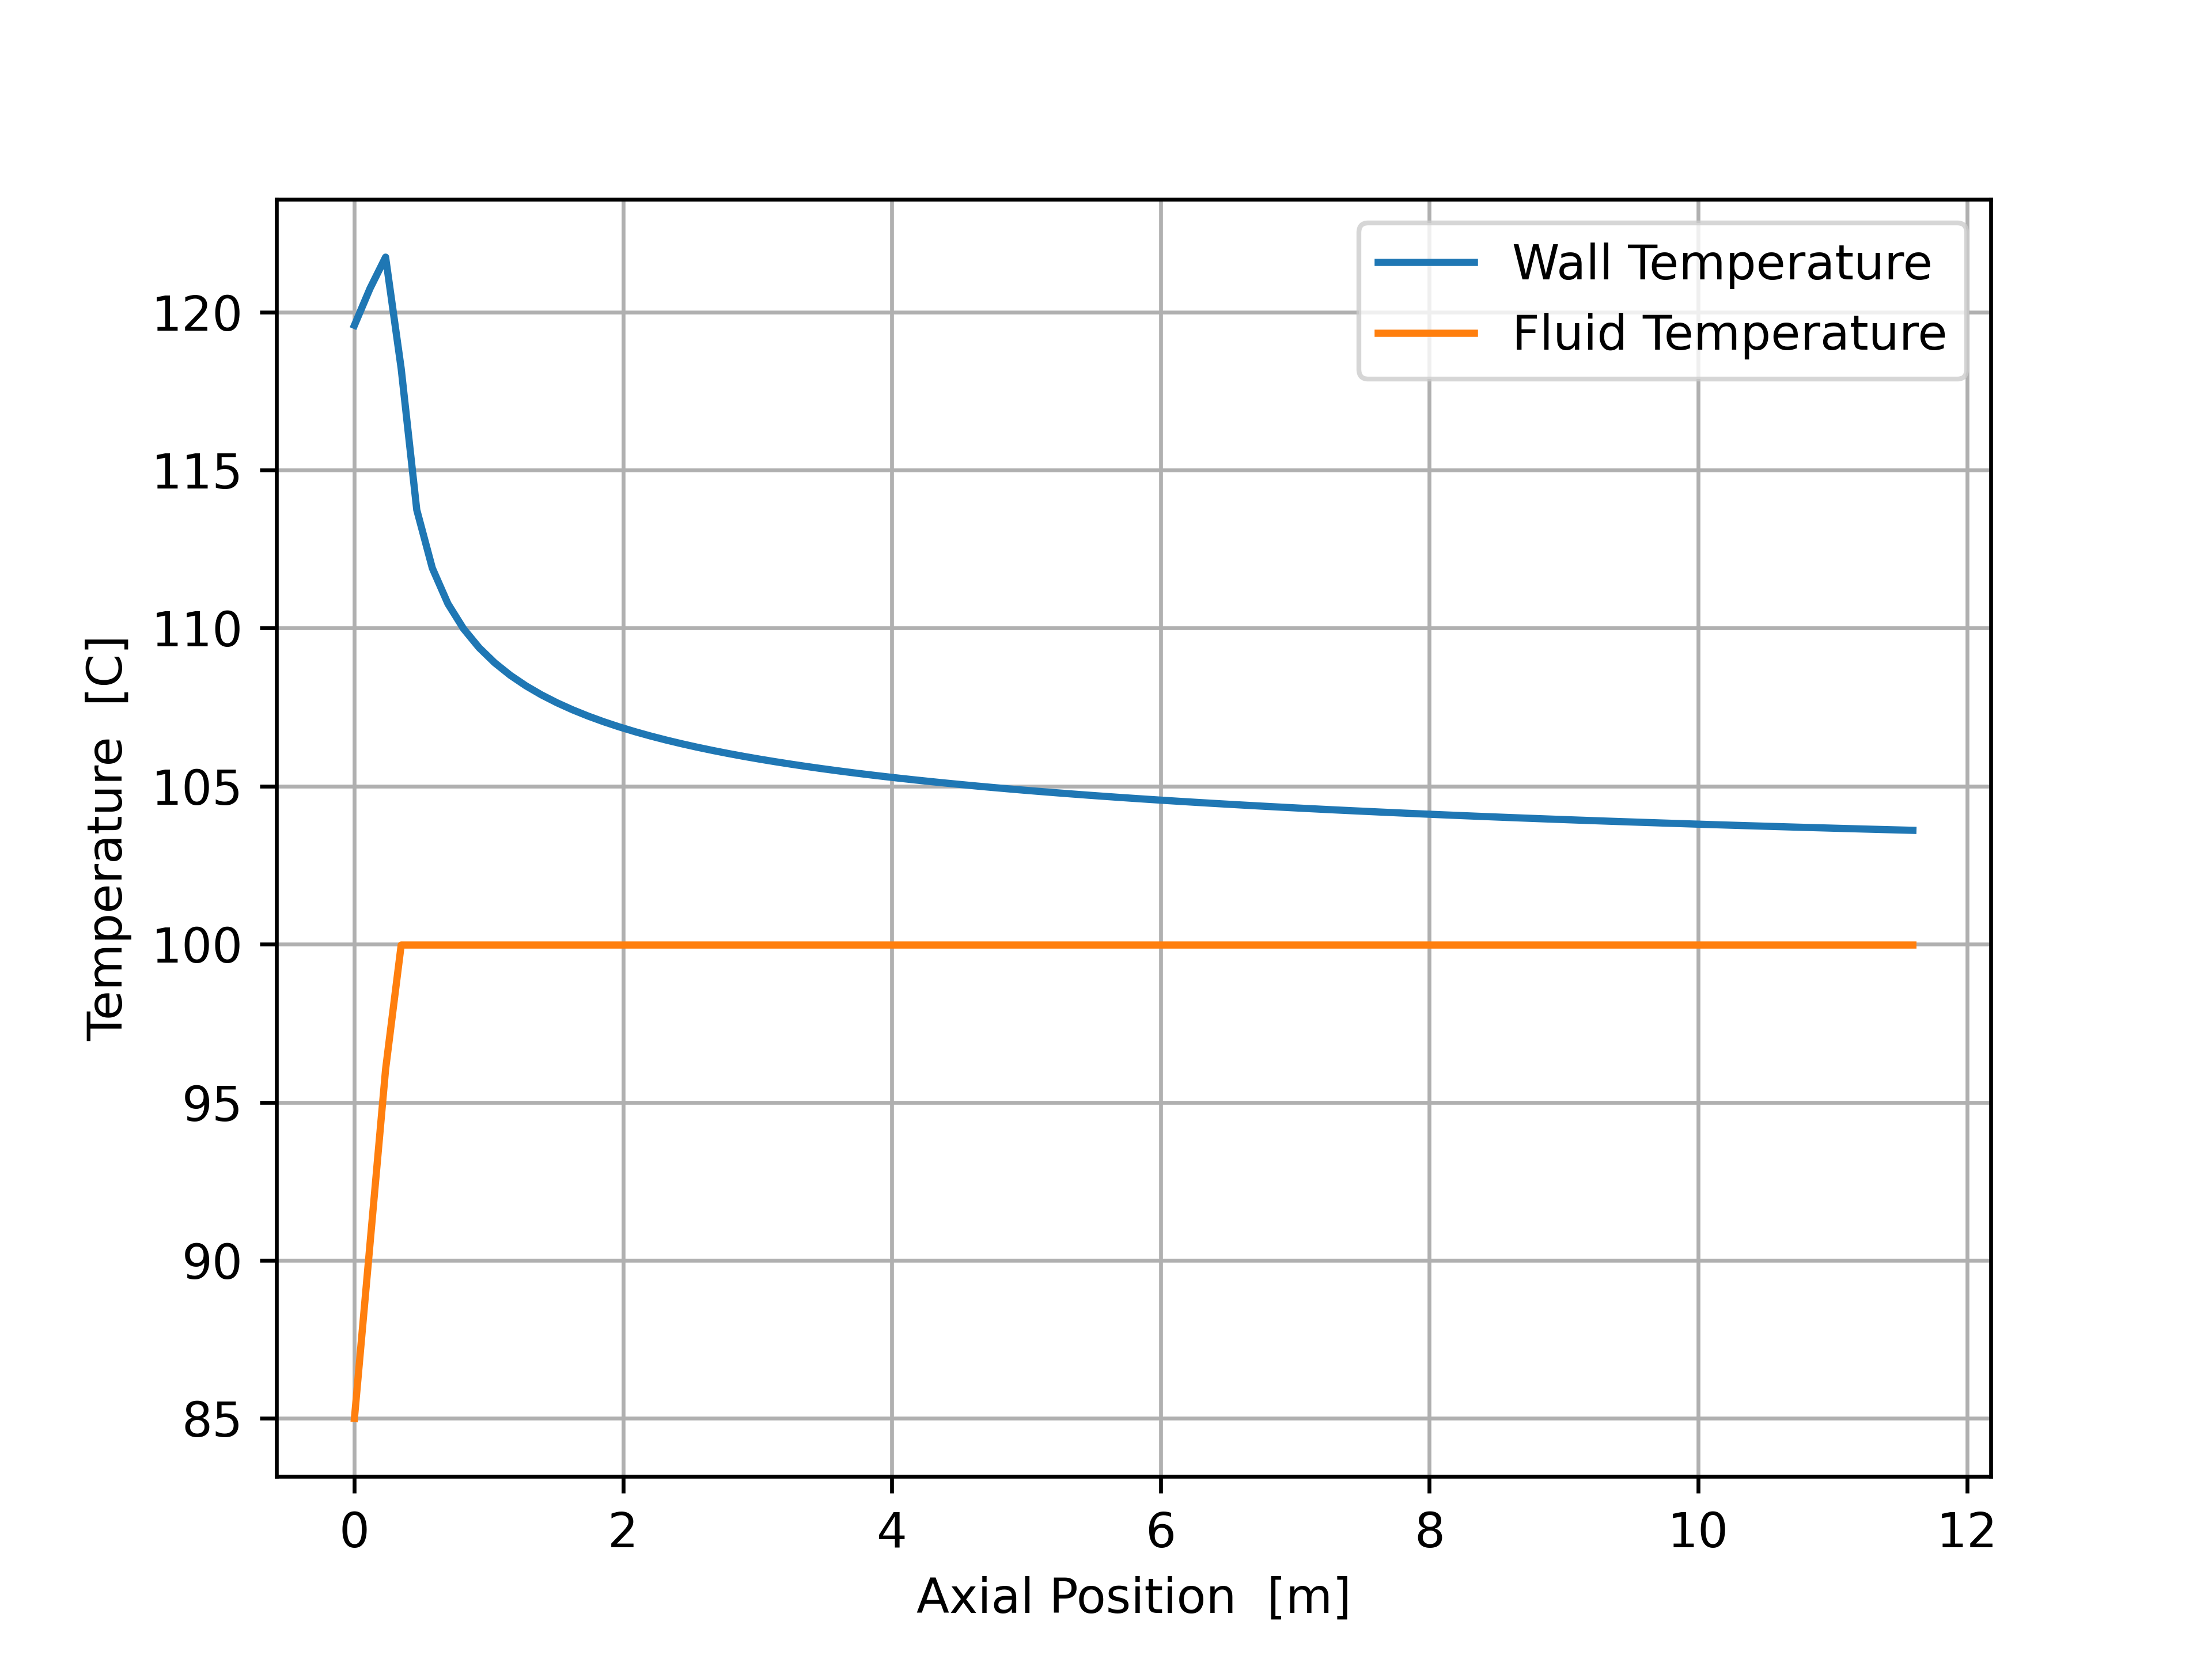
\includegraphics[width=0.5\linewidth]{fig.png}
\end{figure}

\end{document}